\documentclass[a4paper, twoside, 11pt]{report}

%% Language and font encodings
\usepackage[english]{babel}
\usepackage[utf8x]{inputenc}
\usepackage{libertine}
\usepackage{libertinust1math}
\usepackage[T1]{fontenc}

% Reset monospaced font to Computer Modern
\renewcommand{\ttdefault}{cmtt}

% Footnote options
% \counterwithout{footnote}{chapter}

%% Sets page size and margins
\usepackage[a4paper,top=3cm,bottom=2cm,left=3cm,right=3cm,marginparwidth=1.75cm]{geometry}

%% Set line spacing to "one and a half"
\linespread{1.3}

%% Minted syntax highlighting
\usepackage{minted}
\usemintedstyle{emacs}
\setminted{breaklines}
\setminted{fontsize=\small}

%% Useful packages
\usepackage{amsmath}
\usepackage{graphicx}
\usepackage[colorinlistoftodos]{todonotes}
\usepackage[colorlinks=true, allcolors=blue]{hyperref}
\usepackage{xcolor}
\usepackage[justification=centering]{caption}
\usepackage{subcaption}

\title{\texttt{parsley-garnish}: A Linter for the \texttt{parsley} Parser Combinator Library}
\author{Rocco Jiang}
% Update supervisor and other title stuff in title/title.tex

\begin{document}
\begin{titlepage}

\newcommand{\HRule}{\rule{\linewidth}{0.5mm}} % Defines a new command for the horizontal lines, change thickness here

%----------------------------------------------------------------------------------------
%	LOGO SECTION
%----------------------------------------------------------------------------------------


\includegraphics[width=8cm]{title/logo.eps}\\[1cm] % Include a department/university logo - this will require the graphicx package
 
%----------------------------------------------------------------------------------------

\center % Center everything on the page

%----------------------------------------------------------------------------------------
%	HEADING SECTIONS
%----------------------------------------------------------------------------------------

\textsc{\LARGE MEng Individual Project:}\\[0.2cm] % Name of your university/college
\textsc{\LARGE Interim Report}\\[1.5cm]
\textsc{\Large Imperial College London}\\[0.5cm] % Major heading such as course name
\textsc{\large Department of Computing}\\[0.5cm] % Minor heading such as course title

%----------------------------------------------------------------------------------------
%	TITLE SECTION
%----------------------------------------------------------------------------------------
\makeatletter
\HRule \\[0.4cm]
{ \huge \bfseries \@title}\\[0.4cm] % Title of your document
\HRule \\[1.5cm]
 
%----------------------------------------------------------------------------------------
%	AUTHOR SECTION
%----------------------------------------------------------------------------------------

\begin{minipage}{0.4\textwidth}
\begin{flushleft} \large
\emph{Author:}\\
\@author % Your name
\end{flushleft}
\end{minipage}
~
\begin{minipage}{0.4\textwidth}
\begin{flushright} \large
\emph{Supervisor:} \\
Dr. Jamie Willis\\[1.2em] % Supervisor's Name
\emph{Second Marker:} \\
Dr. Robert Chatley % second marker's name
\end{flushright}
\end{minipage}\\[2cm]
\makeatother

% If you don't want a supervisor, uncomment the two lines below and remove the section above
%\Large \emph{Author:}\\
%John \textsc{Smith}\\[3cm] % Your name

%----------------------------------------------------------------------------------------
%	DATE SECTION
%----------------------------------------------------------------------------------------

{\large \today}\\[2cm] % Date, change the \today to a set date if you want to be precise

\vfill % Fill the rest of the page with whitespace

\end{titlepage}

\tableofcontents

\chapter{Introduction}

\section{Motivation}
Parser combinators \cite{hutton_higher-order_1992} are an elegant approach for writing parsers in a manner which remains close to the original grammar specification.
\texttt{parsley} \cite{willis_garnishing_2018} is a parser combinator library implemented as an embedded domain-specific language (\textsc{dsl}) \cite{hudak_building_1996} in Scala, with an API inspired by the \texttt{parsec} \cite{leijen_parsec_2001} family of libraries in Haskell.
However, as with many libraries, there exists a learning curve to utilising \texttt{parsley} and parser combinator libraries in an idiomatic manner.

While well-documented, the wealth of information to get started with \texttt{parsley} can be overwhelming for users, particularly those new to parser combinators.
Furthermore, there exists a number of design patterns \cite{willis_design_2022} for writing maintainable parsers, which even experienced users may be unaware of.
A potential solution to this problem is tooling to provide automated code hints, which a user can use during the development cycle to evaluate if their code adheres to best practices.

% TODO: mention pitfalls of e.g. left recursion here, or in the background? Stuff which can't be picked up by a regular linter

A number of modern integrated development environments (\textsc{ide}s) provide code hints to warn programmers about problems in their source code, highlighting offending snippets and suggesting actions to improve suboptimal or incorrect code \cite{kurbatova_intellij_2021}.
Many of these code analysis tools are designed to detect general issues for the host language, rather than specifically for libraries.
However, tools may also utilise domain-specific code analyses in order to detect issues specific to a particular system or problem domain \cite{renggli_domain-specific_2010,gregor_stllint_2006,xunit_xunitanalyzers_2024}.

This project aims to explore the potential of harnessing code analysis techniques to develop a new tool, \texttt{parsley-garnish}, that offers code hints aimed at assisting programmers in writing idiomatic and correct \texttt{parsley} code.
Additionally, for certain hints which can be automatically fixed, \texttt{parsley-garnish} will provide automated actions to resolve the issue. % TODO: via code transformations - put this in the background?
The goal of \texttt{parsley-garnish} is to be used as a companion library to \texttt{parsley}, in order to improve its ease of adoption and to help users enforce best practices.

\section{Planned Objectives}

\chapter{Static Analysis Tools}

% TODO: might be worth talking about soundness and completeness

% TODO: https://en.wikipedia.org/wiki/Static_program_analysis Cite an article from here maybe
Static program analysis is the process of automatically analysing source code to extract information about its behavior without executing it \todo{cite}, as opposed to dynamic analysis, which is performed on programs as they are run.
Static analysis tools can ease the burden of software development by automating tasks that would otherwise require manual effort and meticulous attention to detail.
These tools can perform a variety of tasks, ranging from detecting possible bugs \cite{johnson_lint_1978,hovemeyer_finding-bugs_2004} to formal software verification of program properties \cite{blanchet_static-analyzer_2003}.

Static analysis tools are increasingly becoming more important in modern software development, as modern code continues to become more complex and difficult to reason about.
Industry leaders, such as Google \cite{sadowski_analysis-google_2018} and Meta (formerly Facebook) \cite{calcagno_moving-facebook_2015}, have embraced static analysis tools as integral components of their software development workflows.

\section{Applications of Static Analysis Tools}
Typically in a software development workflow, multiple static analysis tools are used in conjunction to provide a comprehensive suite of checks.
Often, these tools are integrated into an \textsc{ide} as plugins, allowing them to be consolidated into a single visual interface.

% TODO: is this paragraph now a bit off-topic compared to what is actually discussed?
Refactoring and linting are two major functionalities that these tools provide.
However, because many of these tools include both capabilities, the distinction between them can be blurry.
This section aims to establish definitions for the two terms, which will be used as a basis for subsequent discussion within this thesis.

\subsection{Automated Refactoring}
Code refactoring is a well-established practice in software development.
In his influential book \textit{Refactoring: Improving the Design of Existing Code} \cite{fowler_refactoring_2018}, Fowler defines \textbf{refactoring} as ``the process of changing a software system in such a way that it does not alter the external behavior of the code yet improves its internal structure''.
Refactoring may be employed to eliminate \textbf{code smells}, which are surface indications that could indicate deeper problems in the system.
Code smells are not necessarily problematic on their own, however, they may lead to issues such as bugs or poor maintainability if left unchecked.
Examples of code smells include duplicated code, which can be hard to update without introducing bugs, and long methods, which can be difficult to understand and maintain.
Therefore, it is often productive to refactor code to eliminate code smells, even if the code is still correct and functional.

Static analysis tools can reason about how to safely refactor code in an automated manner, performing refactorings as source-to-source transformations.
These transformations may be implemented as simple text-based replacements or more robust rewrite rules that operate on the abstract syntax tree (\textsc{ast}) of the source code.

Automated refactoring support is particularly useful for large codebases, where manual refactoring would be tedious and error-prone.
Generally, when a user makes use of an automated refactoring tool in an \textsc{ide}, they will manually identify the snippet of code that they wish to refactor, and then select the appropriate refactoring from a list of available options.
Fig.~\ref{fig:extract-function-intellij} presents \textit{Extract Method} \cite{fowler_refactoring_2018} in the IntelliJ IDEA\footnote{\url{https://www.jetbrains.com/idea/}} \textsc{ide}, an example of a common refactoring that can be performed automatically on a block code selected by the user.

\begin{figure}[htbp]
  \centering
  \begin{subfigure}{\textwidth}
    \centering
    \begin{minted}[frame=single,highlightlines={4-5},linenos]{scala}
      object Main {
        def main(args: Array[String]): Unit = {
          val bankDetails = getBankDetails()
          println(s"Account name: ${bankDetails.name}")
          println(s"Account balance: ${bankDetails.balance}")
        }
      }
    \end{minted}
    \caption{A snippet of Scala code. A user may wish to extract the highlighted lines into a separate function.}
    \label{fig:extract-function-intellij-before}
  \end{subfigure}
  \begin{subfigure}{\textwidth}
    \centering
    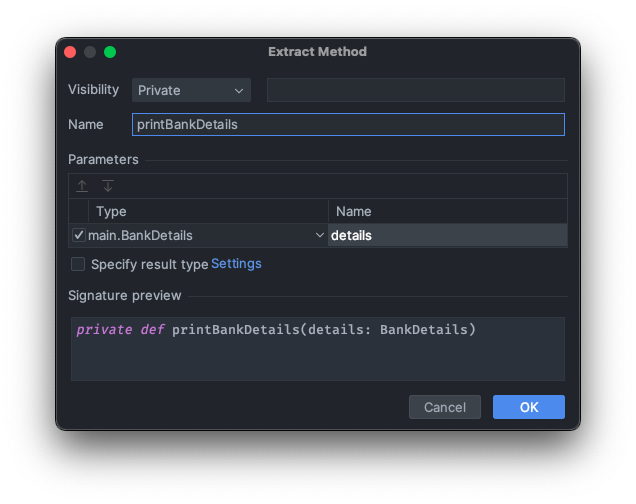
\includegraphics[width=0.75\textwidth]{background/extract-function-intellij.png}
    \caption{When a user selects the highlighted lines from fig.~\ref{fig:extract-function-intellij-before} in IntelliJ IDEA, choosing the \textit{Extract Method} refactoring will open this dialogue to preview changes before applying them.}
    \label{fig:extract-function-intellij-dialogue}
  \end{subfigure}
  \begin{subfigure}{\textwidth}
    \vspace{3ex} % TODO: ew
    \centering
    \begin{minted}[frame=single,highlightlines={4,7-10},linenos]{scala}
      object Main {
        def main(args: Array[String]): Unit = {
          val bankDetails = getBankDetails()
          printBankDetails(bankDetails)
        }

        private def printBankDetails(details: BankDetails): Unit = {
          println(s"Account name: ${details.name}")
          println(s"Account balance: ${details.balance}")
        }
      }
    \end{minted}
    \caption{The result of applying the \textit{Extract Method} refactoring using the chosen parameters in fig.~\ref{fig:extract-function-intellij-dialogue}.}
  \end{subfigure}
  \caption{An example of the \textit{Extract Method} refactoring in IntelliJ IDEA.}
  \label{fig:extract-function-intellij}
\end{figure}

\subsection{Linting}
\textbf{Linting} is the process of analysing source code to identify and report issues related to coding style and potential logical errors.
The term originates from the \texttt{lint} program \cite{johnson_lint_1978}, which examined C source code for bugs, as well as wasteful code patterns that may be legal but error-prone.
The tool was also utilised to enforce portability restrictions which aided users in writing portable code that could be compiled on multiple platforms.
Since the release of \texttt{lint}, many linting tools, known as \textbf{linters}, have been developed for a wide range of programming languages.

Linters are provided as standalone tools separate from a compiler, since their primary goal is to suggest improvements for code readability and maintainability, rather than code optimisations.
Modern linters are commonly integrated into \textsc{ide}s, where code analysis performed by the linter is run incrementally in the background.
Any violations found by the linter are displayed directly in the editor as warnings or errors at the relevant locations in the source code.
This provides an ergonomic user experience, as the user can see the results of the analysis in real-time as part of the development workflow.

Although the strict definition for linting is concerned with only detecting issues in code, many advanced linters today can also provide auto-fixes for violations which can be corrected automatically by static analysis.
% TODO: cite https://link.springer.com/book/10.1007/978-1-4842-7792-8
This auto-fix capability is often integrated into \textsc{ide}s as well: the popular Language Server Protocol for defining \textsc{ide} features enables these auto-fix features via \textit{code actions}.
When a section of code is highlighted by a linter warning, a user can apply a code action to automatically fix the issue with a single click.

Many linters are configurable with a set of rules, which specify the types of issues that the linter should detect.
These rules can be enabled or disabled by the user, allowing them to customise the linter to their needs.
Rules can be categorised by their purpose: some rules are concerned with enforcing code style, while others are concerned with detecting code smells or other suspicious code patterns indicative of possible bugs.

\subsubsection{Style checking and code appearance}
% TODO: CheckStyle https://checkstyle.sourceforge.io/?
% TODO: https://peps.python.org/pep-0008/
Linters can be configured to enforce a particular style guide defining a set of conventions for how idiomatic code should be written.
They can highlight style violations and in basic cases, automatically rewrite code to conform to the correct style.
For example, the \textit{Flake8}\footnote{\url{https://flake8.pycqa.org/en/latest/}} linter for Python enforces coding conventions from the PEP 8 style guide \todo{cite}.
Stylistic rules are especially helpful for large projects with multiple contributors, where a consistent coding style can improve readability and maintainability.

\subsubsection{Identifying opportunities for refactoring}
Certain linting rules can aid in the refactoring process by broadly identifying code smells and candidate areas for refactoring, suggesting appropriate actions that the user can take.
As an example, a linter may detect a fragment of code that is repeated in multiple places: this is a code smell, as discussed previously.
The linter may then suggest a code action to automatically apply the \textit{Extract Method} refactoring to avoid code duplication.

\subsubsection{Suggesting idiomatic usage}
Other rules can suggest opportunities to improve more precise snippets of code by utilising language features in a more idiomatic manner.
These rules are especially helpful for new users of a language, who may be unaware of useful language constructs and idioms.
% TODO: Clippy for Rust https://arxiv.org/abs/2310.11738
For example, the \textit{Clippy}\footnote{\url{https://doc.rust-lang.org/clippy/}} linter for Rust \todo{cite article} categorises a collection of rules as \texttt{clippy::complexity} rules to detect code that does something simple in a complex way and suggests a simpler alternative.
Fig.~\ref{fig:hlint-example} provides an example of a similar rule in Haskell, from the \textit{HLint}\footnote{\url{https://hackage.haskell.org/package/hlint}} linter.
The rule suggests an $\eta$-reduction refactoring, presented to the user as a code action that can be applied automatically.

\begin{figure}[htbp]
  \vspace{3ex} % TODO: make this less hacky
  \centering
  \begin{subfigure}{0.45\textwidth}
    \centering
    \begin{minted}[frame=single]{haskell}
      foo xs = map (+1) xs
    \end{minted}
    \caption{A Haskell function \texttt{foo}, which can be made more concise using $\eta$-reduction.}
  \end{subfigure}
  \hfill
  \begin{subfigure}{0.45\textwidth}
    \centering
    \begin{minted}[frame=single,escapeinside=||]{text}
      Eta reduce
      Found:
        foo xs = map (+ 1) xs
      Why not:
        foo = map (+ 1)
      |\textcolor{gray}{hlint(refact:Eta reduce)}|
    \end{minted}
    \caption{The linter warning shown for \texttt{foo}.}
  \end{subfigure}
  \caption{An example of a warning from the Haskell linter \texttt{hlint}, suggesting a fix that a user can choose to automatically apply.}
  \label{fig:hlint-example}
\end{figure}

Many idiomatic practices exist to avoid common pitfalls that may lead to unintended behaviour.
By highlighting good practices, linters can help users avoid these common mistakes that may cause bugs.
For example, \textit{ESLint}\footnote{\url{https://eslint.org/docs/latest/rules/}}, one of the most popular JavaScript linters, warns against common JavaScript pitfalls such as using the regular equality operator \texttt{==} instead of its type-safe alternative \texttt{===}.

Linters developed for a specific library provide rules to enforce idiomatic usage specific to the domain of the library.
% TODO: is this the paper that talks about this? https://ieeexplore.ieee.org/abstract/document/6405305/references#references
A library or especially an embedded \textsc{dsl} may require a particular style of usage that is different from the host language.
Therefore, a regular linter for the host language may not be able to detect issues specific to the library.
In this case, an accompanying linter can greatly benefit users: common misuses can be detected and sometimes automatically fixed, and users can be directed to relevant documentation to learn more about correct usage.
For instance, the \textit{xUnit.net} testing framework for C\# is accompanied by the \texttt{xunit.analyzers}\footnote{\url{https://github.com/xunit/xunit.analyzers}} package which provides linting rules to enforce best practices specific to xUnit.

\subsubsection{Detecting potential bugs}
Linters may also directly attempt to detect more serious issues in code, such as possible logic errors.
This can be helpful for even experienced users to avoid common pitfalls.
Clippy has \texttt{clippy::suspicious} and \texttt{clippy::correctness} rule categories to identify code that is very likely to be incorrect or useless.
ESLint provides several rules to warn against code patterns that are likely to cause runtime errors, such as re-assigning a \texttt{const} variable.

\section{Static Analysis for Scala}
\subsection{Choice of Tooling}
The goal of \texttt{parsley-garnish} is to provide linting and refactoring capabilities for the \texttt{parsley} parser combinator library.
Since \texttt{parsley} is a Scala library, this project must be implemented using a tool capable of statically analysing Scala code.
This section will therefore discuss and evaluate the choices available for implementing \texttt{parsley-garnish}.

\subsubsection{Scala compiler plugins}
% TODO: cite https://dl.acm.org/doi/abs/10.1145/3331545.3342599
The most powerful approach would be to implement \texttt{parsley-garnish} as a compiler plugin \todo{cite}.
Using the low-level compiler \textsc{api}, it is possible to perform arbitrary code transformations at any step of the compilation process.
Compiler plugins therefore offer full freedom to extend the Scala compiler with extra functionality, such as extra passes for code analysis and emitting lint warnings as diagnostics or even compiler errors.

However, this approach has several drawbacks.
Firstly, compiler plugins are tightly coupled with the compiler itself, and therefore not portable across major compiler versions.
% https://github.com/mattmoore/scala-compiler-plugins is a good reference, in case I need to revisit this
% TODO: cite https://docs.scala-lang.org/scala3/reference/changed-features/compiler-plugins.html (probably the latter)
For instance, plugins written for the Scala 3 compiler, known as \texttt{dotty}, are completely incompatible with Scala 2 plugins \todo{cite}.
Additionally, developing compiler plugins requires a deep understanding of arcane and poorly documented compiler internals.
% TODO: cite https://link.springer.com/chapter/10.1007/978-3-662-46663-6_2
Exposing the full compiler \textsc{api} permits unsafe operations that may violate undocumented invariants assumed by the compiler, leading to exceptions during compilation or even malformed bytecode \todo{cite}.
The lack of higher-level abstractions also makes it difficult to implement even trivial tasks such as renaming a field.

For these reasons, it would be preferable to explore other tools that may use compiler plugins themselves but provide a higher-level interface for implementing code analysis and transformations.

\subsubsection{Scalameta}
\textit{Scalameta}\footnote{\url{https://scalameta.org/}} is a metaprogramming framework for Scala that provides a unified interface for performing common metaprogramming tasks.
It provides a high-level syntactic \textsc{api} for transforming and pretty-printing Scala source code, as well as a semantic \textsc{api} providing access to semantic information such as type inference and name resolution.
% TODO: cite https://infoscience.epfl.ch/record/226166
Scalameta is the successor of the earlier \texttt{scala.reflect} metaprogramming framework, which parsed source code into lossy trees that discarded syntactic information such as comments and whitespace \todo{cite}.
On the other hand, Scalameta trees are lossless and preserve all syntactic details, a key feature that allows code transformations and refactorings to preserve formatting details.

% TODO: cite https://inthisbuild.readthedocs.io/en/latest/index.html. See GitHub source code for date information.
Scalameta's semantic \textsc{api} is powered by \textit{SemanticDB}, a compiler-agnostic data model for semantic information in Scala programs \todo{cite}.
This allows Scalameta to extract semantic information via compiler plugins that emit data in the SemanticDB format.
Thus, Scalameta can work with any compiler that supports SemanticDB, rather than being tied to a specific compiler implementation.

Since Scalameta provides a high-level interface for manipulating syntactic and semantic information, it is a promising choice for this project.
Being able to access semantic information is especially helpful for implementing more complex code analyses.
However, Scalameta's primary focus is on providing a general metaprogramming framework and therefore lacks \textsc{api} support specifically for implementing linting and refactoring rules.
For example, the Scalameta tree transformation utilities do not preserve formatting details when pretty-printed, despite the underlying trees containing this information.

\subsubsection{Scalafix}
\textit{Scalafix}\footnote{\url{https://scalacenter.github.io/scalafix/}} is a refactoring and linting tool built on top of Scalameta.
It specifically provides an \textsc{api} for implementing fine-grained code transformations that preserve comments and formatting details.
% TODO: cite https://www.scala-lang.org/blog/2017/09/11/scalafix-v0.5.html
Scalafix provides a framework for implementing linting rules to emit warnings, as well as rewrite rules to perform automated code transformations \todo{cite}.
Since it is built on Scalameta, a major advantage of Scalafix is that it is also compiler-agnostic and could be integrated into any \textsc{ide} if a plugin is developed for it.

% TODO: cite https://scala-lang.org/blog/2016/10/24/scalafix.html
Originally, Scalafix was designed to help automate the process of migrating code from Scala 2 to 3, which involved many breaking changes to the language \todo{cite}.
However, Scalafix has since evolved into a general-purpose tool for implementing code transformations and analyses, utilising the powerful syntactic and semantic \textsc{api}s provided by Scalameta.
Scalafix rules can be either syntactic or semantic, depending on whether they require semantic information to perform their analysis.
Syntactic rules are faster to run, since they operate purely on the \textsc{ast} without requiring compilation to extract semantic information, but are more limited in the accuracy of analyses they can perform.

Scalafix is growing to become the de-facto modern successor to earlier refactoring tools such as Abide\footnote{\url{https://contributors.scala-lang.org/t/whats-the-status-of-abide/}} and \texttt{scala-refactoring}\footnote{\url{https://github.com/scala-ide/scala-refactoring}}.
\texttt{scala-refactoring} used \texttt{scala.reflect} to implement code transformations, with much extra work utilising the Scala Presentation Compiler \textsc{ast} to preserve formatting details lost by \texttt{scala.reflect}.
As a result, maintaining the library became difficult and the project was abandoned in favour of a clean implementation using Scalameta, which was designed in part to address the shortcomings of \texttt{scala.reflect}.

A drawback of Scalafix is that it is primarily a command-line tool, and therefore by default does not provide a user-friendly interface for interactive usage.
However, this can rectified in the future by integrating Scalafix into the Metals \textsc{lsp} server for Scala, which would allow it to be integrated into any \textsc{ide} that supports the LSP.

Overall, Scalafix emerges as the most favorable choice for implementing \texttt{parsley-garnish}.
It provides high-level \textsc{api}s specifically for implementing linting and rewrite rules without necessitating extensive knowledge of compiler internals.
Scalafix is also being actively developed and maintained, with good basic documentation and a growing number of examples of usage in the wild.

\subsubsection{Other tools considered}
The main alternate contender to Scalafix is the IntelliJ Scala Plugin\footnote{\url{https://github.com/JetBrains/intellij-scala}}.
However, while the plugin offers superior interactive usage within the IntelliJ IDEA \textsc{ide}, it is tied to the IntelliJ Scala compiler and therefore not portable across other compilers.
To maintain flexibility and not tie \texttt{parsley-garnish} to a particular compiler or code editor, Scalafix is a preferable option.
Furthermore, documentation is less clear on how to write a Scala plugin for IntelliJ compared to the Scalafix documentation.

WartRemover\footnote{\url{https://www.wartremover.org/}} is a linter implemented as a compiler plugin, with support for writing custom rules.
However, it only can emit warnings or errors and does not support auto-fixes, making it less suitable for \texttt{parsley-garnish}'s goals.

ScalaStyle\footnote{\url{http://www.scalastyle.org/}} is primarily a style checker which also supports custom rules.
However, it is only able to perform syntactic analyses and does not have access to semantic information, restricting the types of analyses it can perform.

% TODO: maybe a section introducing ScalaFix and how it works? or is that too much detail?
% TODO: maybe a figure to show an example of a ScalaFix rewrite rule?

\chapter{Parser Combinators}

\chapter{Project Plan}
\section{Proposed deliverables and milestones}
This project is rather exploratory in nature, and as such, these milestones are highly subject to change as the project progresses.
However, I have attempted to outline some key deliverables which I believe to be achievable, as well as some optional deliverables to explore if time permits.

\subsection{Key deliverables}
\begin{itemize}
  \item
  Simple lint rules for non-idiomatic combinator usage which can be simplified with an automated refactoring.
  For example, \texttt{endBy(p, sep)} is the idiomatic equivalent to \texttt{many(p <* sep)}.
  \item
  Detection of left-recursive parsers, which are a bug pattern since they will cause infinite recursion at runtime.
  It should be possible to perform a static analysis to produce a code transformation to utilise the \texttt{postfix} family of combinators to eliminate left-recursion and resolve the bug.
  \item
  Lint rules to detect ambiguity in parsers, which can be a bug pattern since the parser may not behave as expected.
  It may be possible to provide an automated fix in some cases, but more research has to be done to determine the feasibility of this.

  Conversely, it may also be possible to detect overuse of the \texttt{atomic} combinator.
  Users may overuse this combinator to avoid ambiguity, but overuse is a code smell as it can negatively impact error messages reported by the parser.
  \item
  Proofs that all code transformations preserve the semantics of the original parser.
\end{itemize}

\subsection{Optional deliverables}
\begin{itemize}
  \item
  Lint rules that warn against side-effecting parsers.
  \texttt{Parsley} employs aggressive parser optimisations which may assume that parsers are pure.
  The lint rule would remind users to use the \texttt{impure} combinator to avoid \texttt{parsley} from optimising away any intended behaviour.
  \item
  Lint rules to detect when a parser using \texttt{chain/infix/postfix} combinators can be rewritten to use a precedence table, and the automated refactoring to accompany this rule.
  Further lints/refactorings related to precedence tables may also be possible, such as looking at type information to determine the most appropriate shape (\texttt{Ops/SOps/GOps}).
  \item
  An editor plugin or extension to provide integration of \texttt{parsley-garnish} into the code editor.
  As explored in the background section, it is possible to provide this integration for Scalafix, but the difficulty of this task is unknown.
  \item
  Exploration of possible pedagogical applications of \texttt{parsley-garnish}.
  For example, lint rules may be useful for marking submissions for the Second Year WACC compilers project.
\end{itemize}

\section{Current Progress}
Most of the work so far has been on research and experimentation with Scalafix.
Although there was good documentation to get started, Scalafix is an active project and the documentation is not always fully comprehensive or up-to-date.
I still have some concerns about whether the Scalafix \textsc{api} is expressive enough to implement all of the analyses I have in mind, but I will continue to explore this as the project progresses.

From my experimentation, I have a relatively good idea of how to implement most of the ``simple'' lint rules.

At the time of writing, I have also implemented a proof-of-concept rule for transforming left-recursive parsers, on a small subset of \texttt{parsley}'s combinators.
This has been encouraging but much work remains to be done to be able to apply the rule on more complex parsers.
The current results of the transformations are also sometimes too complex, so I will need to investigate methods such as defunctionalisation and/or alternate methods of representing terms to simplify the output statically.
Furthermore, the transformation is likely to be correct but not proven yet.

\section{Project Timeline}

My immediate plan is to continue work on the left-recursion transformation, while also working on the simpler lint rules.
I hope to complete the left-recursion rule by early March, although unforseen difficulties may arise (such as if output simplification proves to be more difficult than expected).
If it is not complete or close to complete by then, I will re-evaluate the feasibility of the rest of the milestones and adjust accordingly.
I have already communicated to my supervisor that this left-recursion rule will likely be the most involved deliverable of the project, although there is also a chance that many of the techniques employed could be reused for other transformations.

The next two months will be spent exploring other milestones.
I plan on approaching this by alternating research and implementation, as I have found that this has been a good way to make progress so far, while also guaranteeing that I will make progress on the final deliverable.

By the beginning of summer term, I would also like to have a very rough draft of the final report completed, based on the work completed so far.
This will allow me to communicate with my supervisor on the state of the project, as well as leaving me ample time to edit and refine the report.
The remaining milestones to cover will be decided during this meeting; at this point, having implemented a number of rules, I hope to have a much better grasp on how long each deliverable could take.
This remaining time will then be divided between writing the report and implementing the agreed-upon milestones.

\chapter{Evaluation Plan}

A large corpus of student WACC parsers is available to evaluate the real-world applicability of \texttt{parsley-garnish}.
This can be utilised to assess the tool's ability to achieve quantitative and qualitative metrics.

The large number of parsers available to test can help evaluate the correctness and accuracy of each lint rule.
We might find that certain rules are more prone to false positives than others, or that some automated refactorings may introduce new issues such as compilation errors.
These quantitative metrics can be counted and used to evaluate rules against each other, as well as the overall effectiveness of the tool.

We can also estimate the proportion of issues that \texttt{parsley-garnish} is able to detect automatically.
This can be done by comparing the number of issues detected automatically against the number of issues found manually by a code reviewer.

Qualitative metrics such as the quality of automated fixes can also be assessed by manually reviewing the output of the tool.
For example, an issue I pointed out in the project plan is that the output of the left-recursion transformation may be in a form that is ``ugly'' when it could be simplified to a much more human-readable form.
The quality of fixes would affect the practicality of the \texttt{parsley-garnish}, since users may be reluctant to apply automated fixes if the output quality can be poor.

Furthermore, the performance of \texttt{parsley-garnish} can be evaluated in terms of execution time and resource consumption.
There are no direct competitors to benchmark against, but we can still evaluate the tool's performance against a baseline of acceptable performance, or perhaps a collection of other Scala static analysis tools deemed to be of similar complexity.
I am thinking of benchmarking the tool during development as well, since it may affect design decisions such as implementing some rules as purely syntactic rather than semantic rules.
I am not sure how much resource overhead a semantic rule would incur, so this could be insignificant or a major tradeoff (between speed, correctness, and accuracy) to consider.

Finally, it is possible to gather feedback from students interested in using \texttt{parsley-garnish} to improve their WACC parsers.
User surveys and interviews would provide insights into the tool's usability, helpfulness, and areas for improvement.
Although the timing of the WACC Lab does not align with the project timeline, I am hoping that some students may still be interested in trying out the tool on their final WACC submissions or possibly personal projects using \texttt{parsley}.
% \chapter{Conclusion}
% \appendix
\chapter{First Appendix}

\bibliographystyle{vancouver}
\bibliography{bibs/parsers,bibs/tools,bibs/misc}

\end{document}